\chapter{ Выполнение работы}
\label{cha:analysis}

\section{ Первое задание}
Представить следующие списки в виде списочных выражений:

\begin{figure}[ht!]
    \centering{
        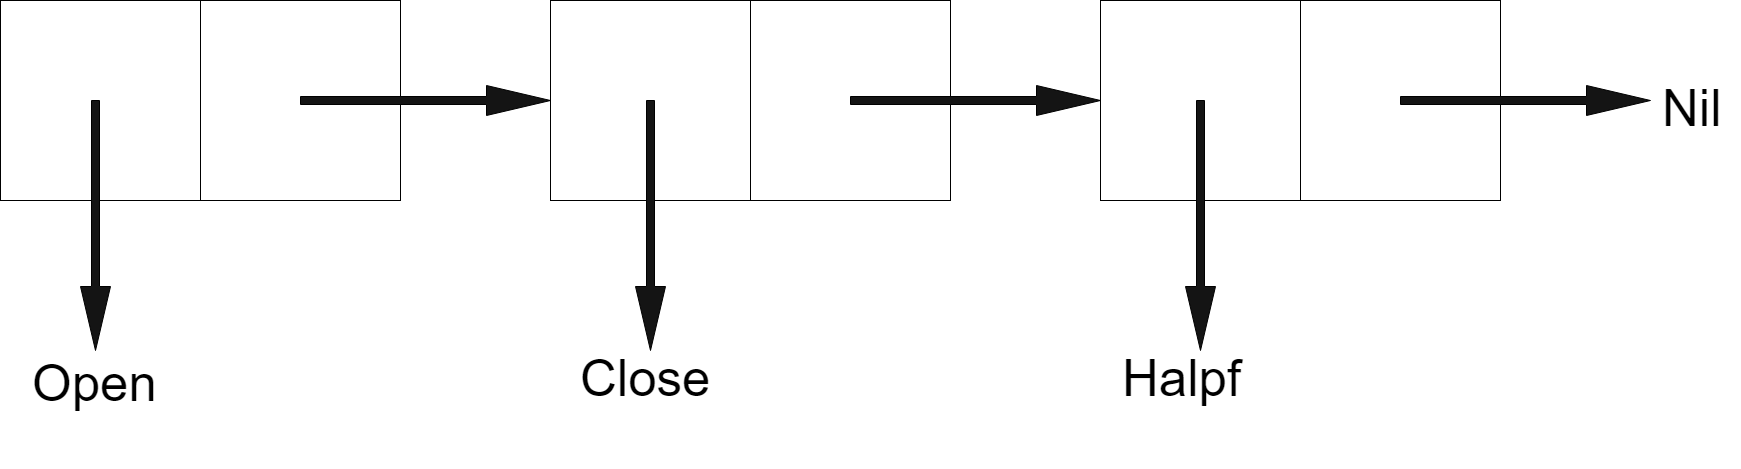
\includegraphics[width=1\textwidth]{img/OpenCloseHalpf.png}
        \caption{ Представление выражения `(open close halph) в виде списочных ячеек}
        \label{fig:openclosehalph}
    }
\end{figure}

\begin{figure}[ht!]
    \centering{
        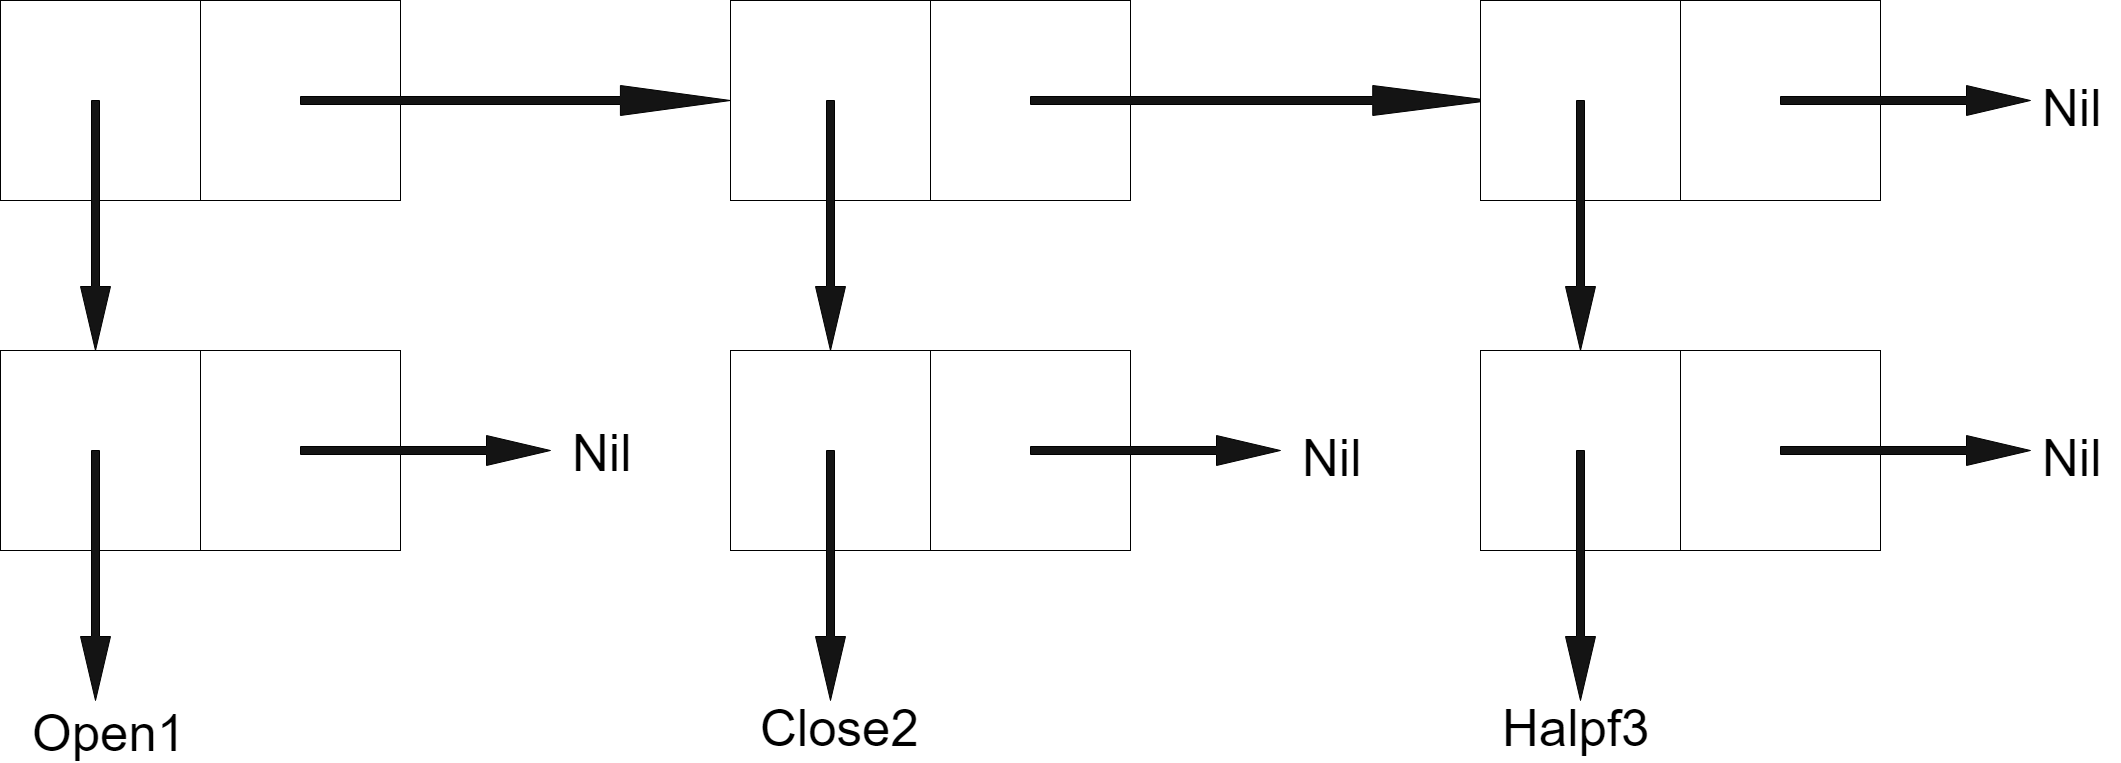
\includegraphics[width=1\textwidth]{img/Open1Close2Halpf3.png}
        \caption{ Представление выражения `((open1)(close2)(halph3)) в виде списочных ячеек}
        \label{fig:open1close2halph3}
    }
\end{figure}

\begin{figure}[ht!]
    \centering{
        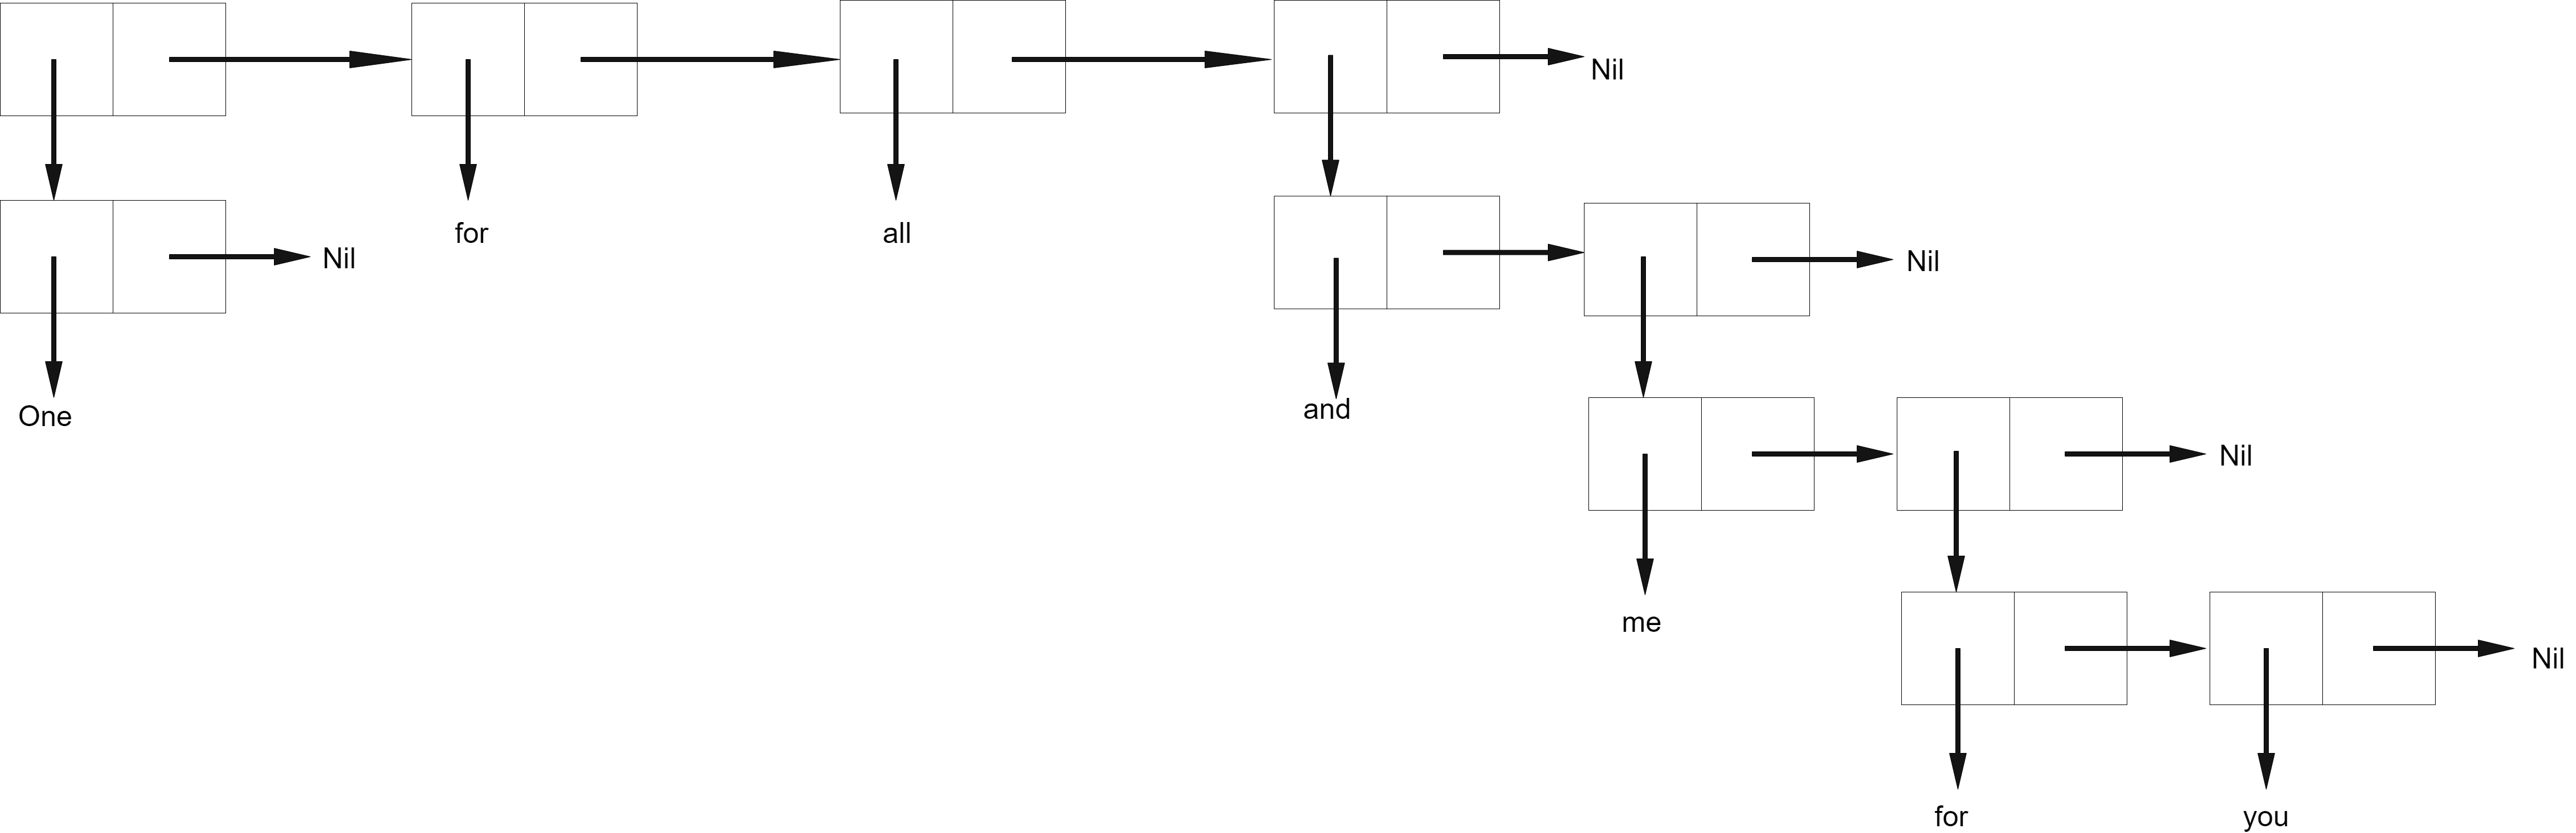
\includegraphics[width=1\textwidth]{img/OneForAllAndMeForYou.png}
        \caption{ Представление выражения `((one)for all (and(me(for you)))) виде списочных ячеек}
        \label{fig:oneforall}
    }
\end{figure}

\begin{figure}[ht!]
    \centering{
        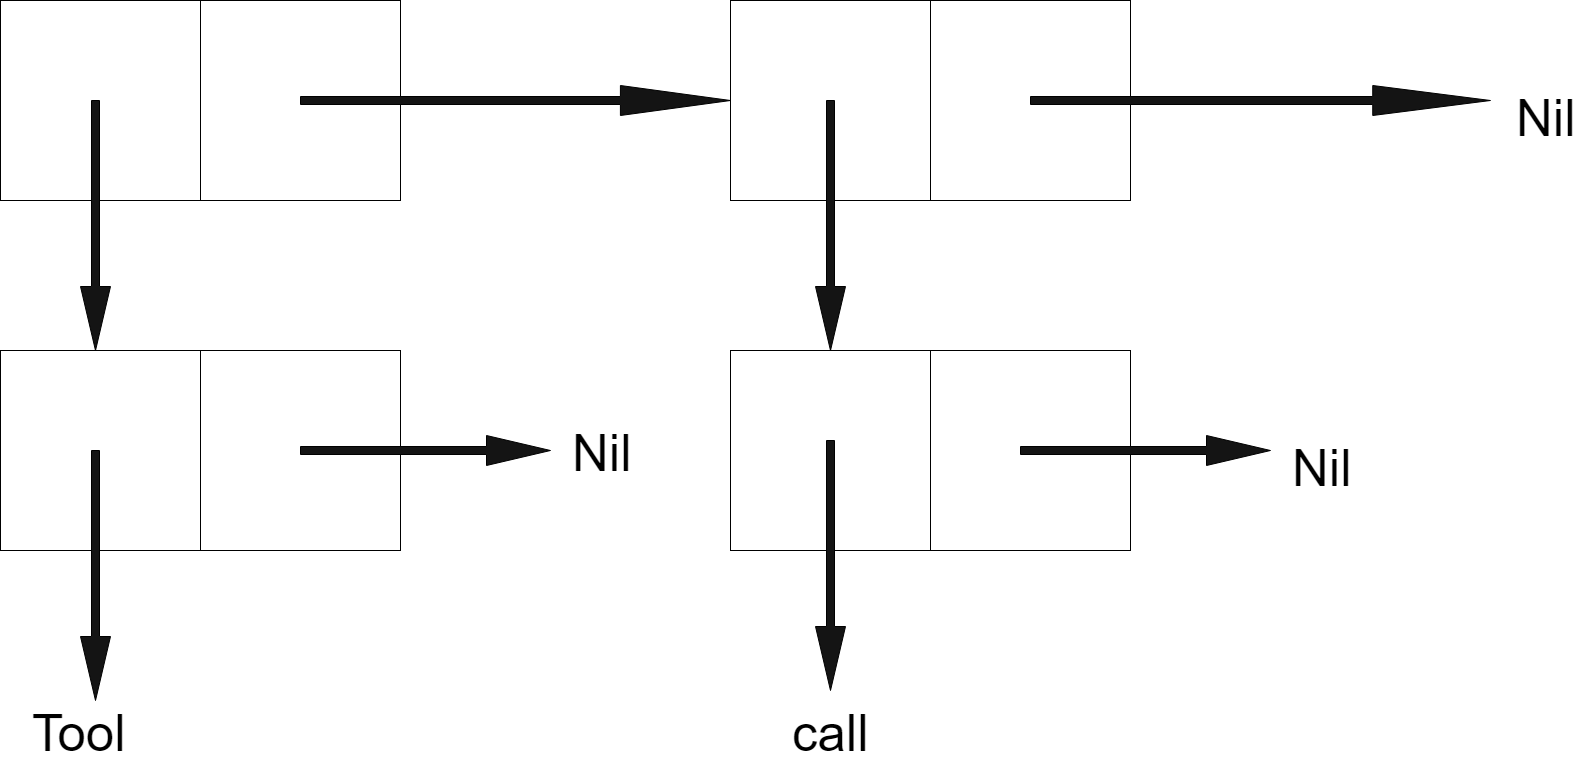
\includegraphics[width=1\textwidth]{img/ToolCall.png}
        \caption{ Представление выражения `((TOOL)(call)) в виде списочных ячеек}
        \label{fig:toolcall}
    }
\end{figure}

\begin{figure}[ht!]
    \centering{
        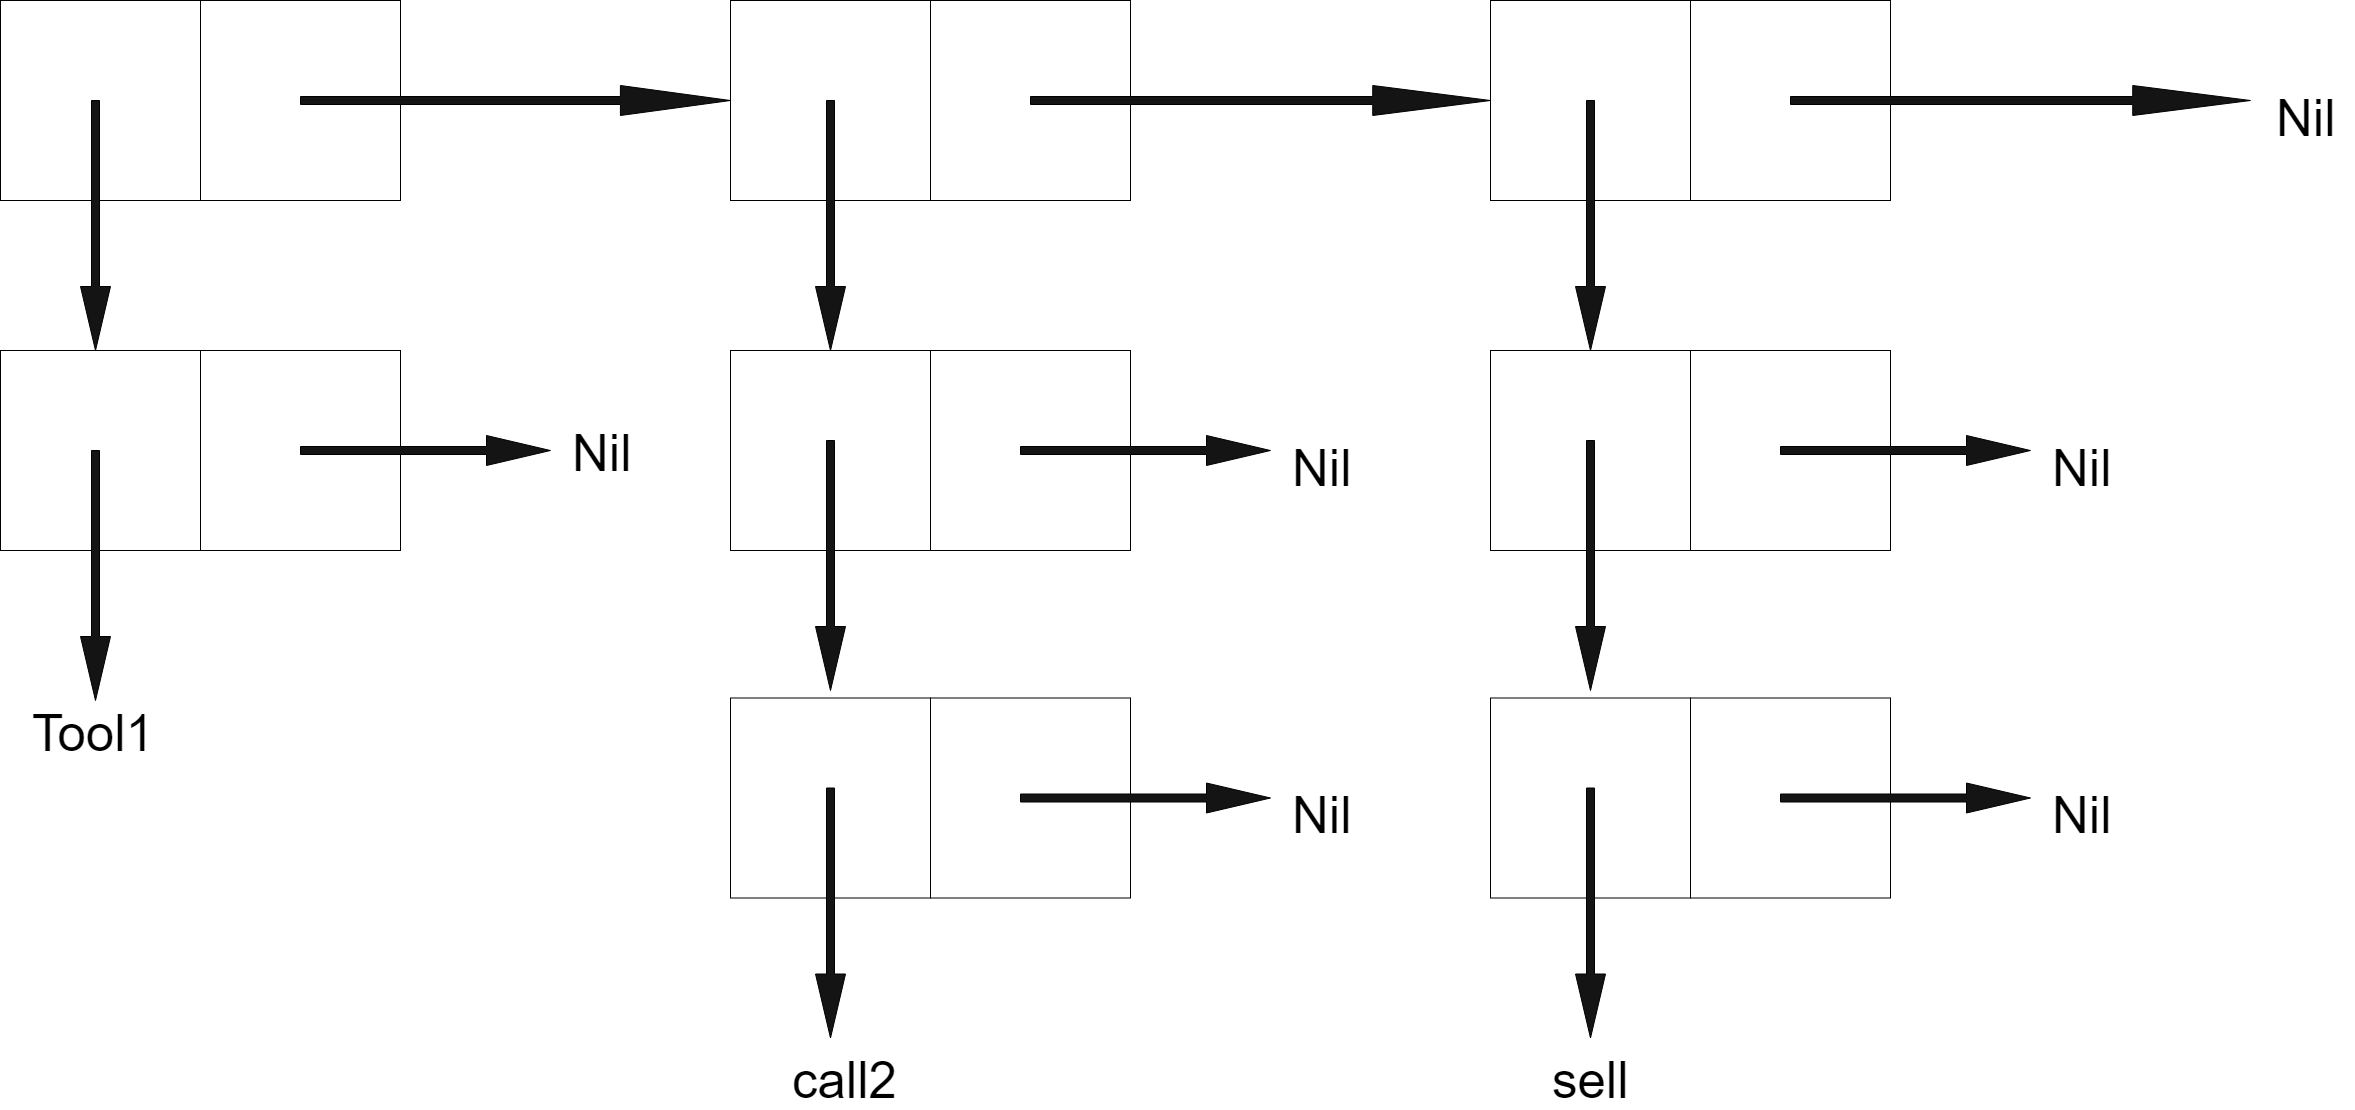
\includegraphics[width=1\textwidth]{img/Tool1Call2Sell.png}
        \caption{ Представление выражения `((TOOL1)((call2))((sell))) в виде списочных ячеек}
        \label{fig:tool1call2sell}
    }
\end{figure}

\begin{figure}[ht!]
    \centering{
        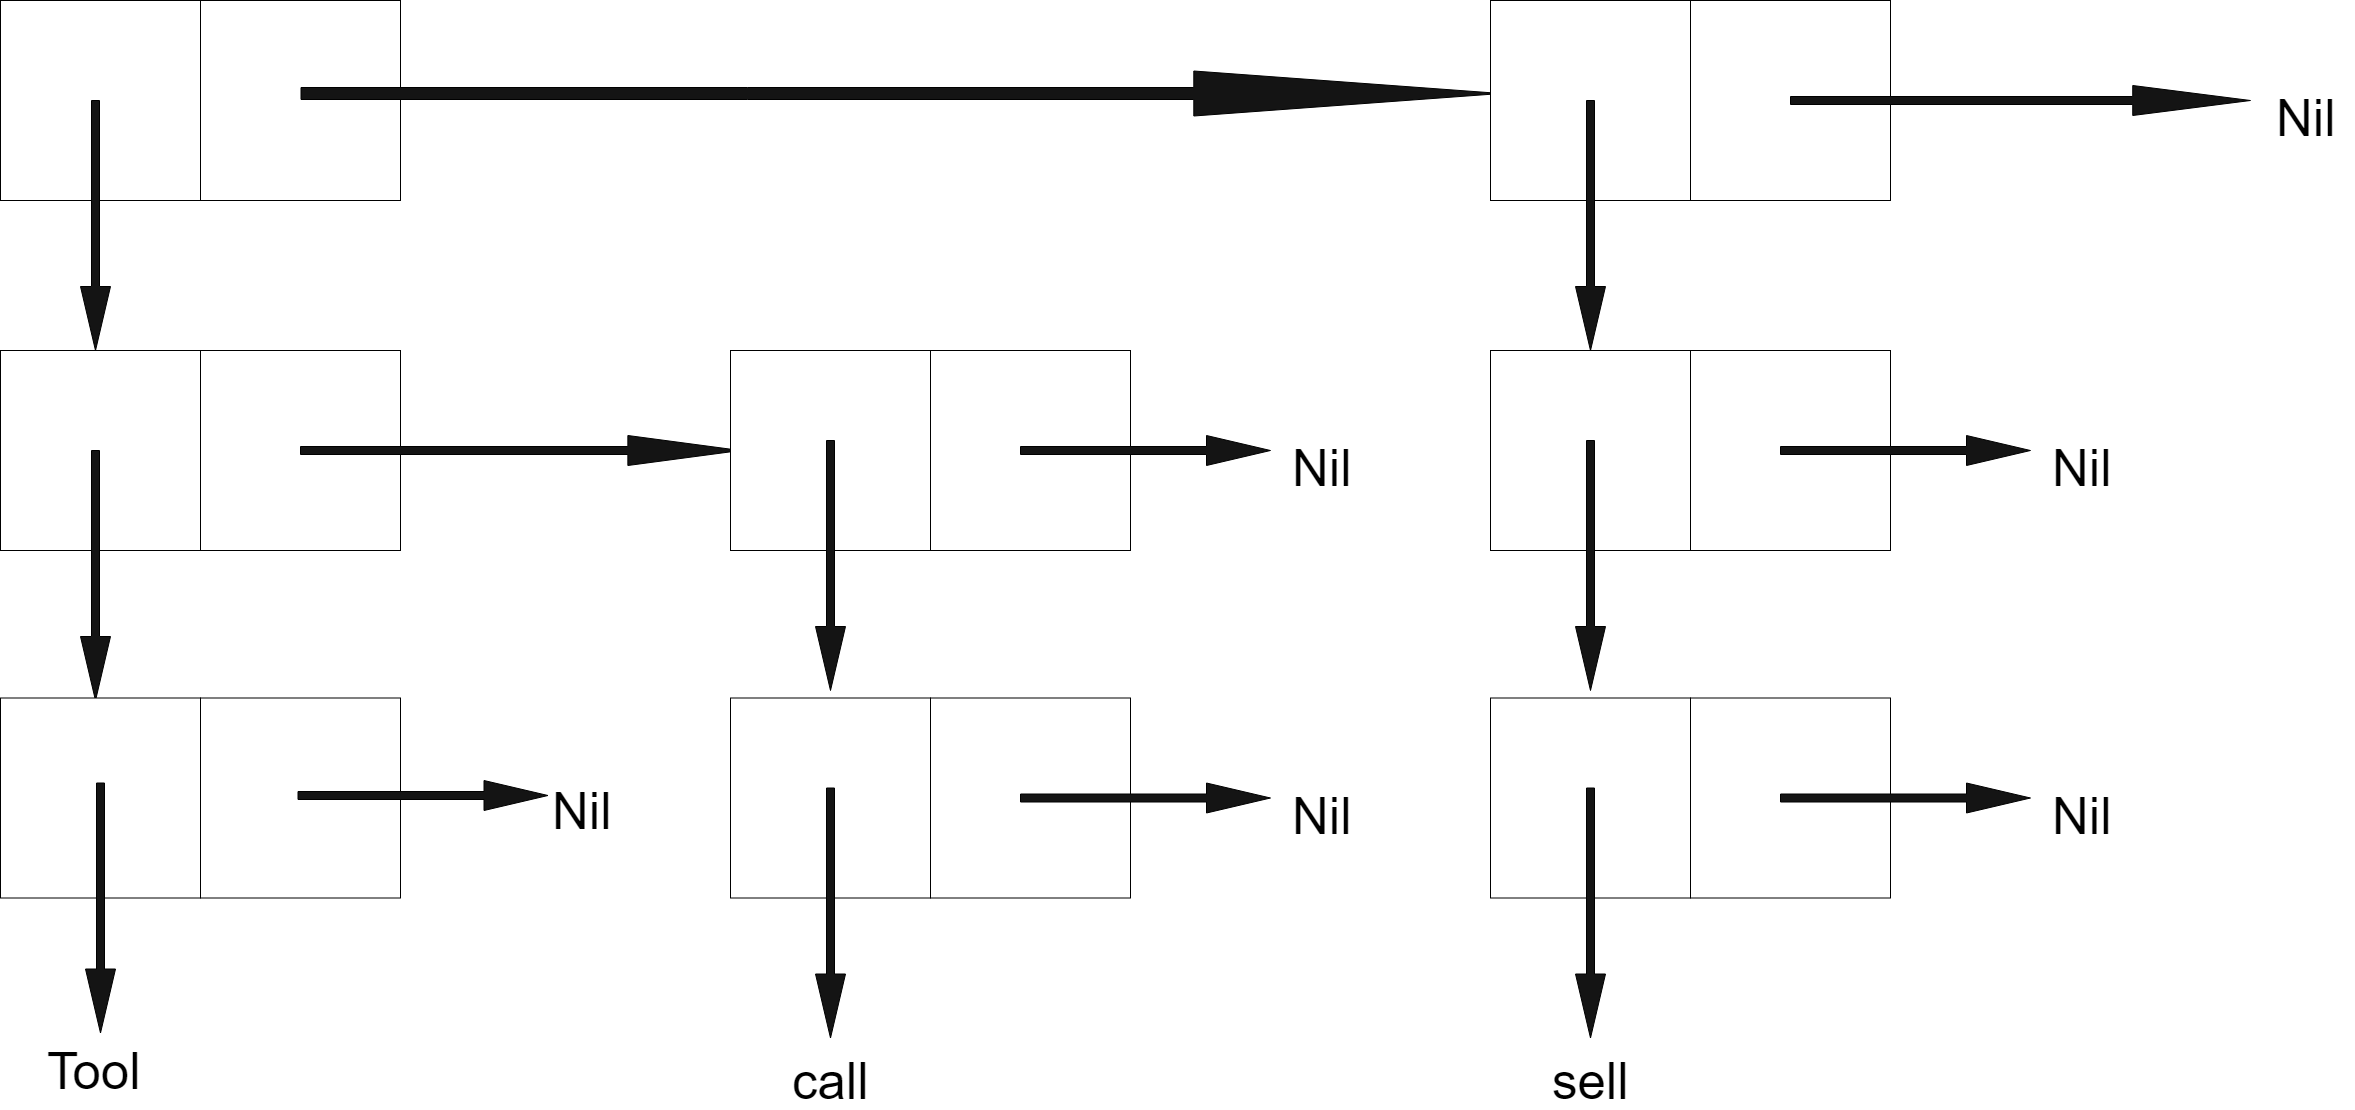
\includegraphics[width=1\textwidth]{img/ToolCallSell.png}
        \caption{ Представление выражения `(((TOOL)(call))((sell))) в виде списочных ячеек}
        \label{fig:toolcallsell}
    }
\end{figure}

